%------------------
%	PACKAGES AND DOCUMENT CONFIGURATIONS
%------------------

% Original template  https://www.overleaf.com/latex/templates/template-for-foundation-master-project-reports/dtzztzckwswh

% 12 point
\documentclass[a4paper,12pt]{article} % preamble - found size is defined within this tag
% Times New Roman
\usepackage{tgtermes}
% single line space - latex default
% \linespread{1}

% Adjusting margins to personal my need
\addtolength{\oddsidemargin}{-.5in}
\addtolength{\evensidemargin}{-.5in}
\addtolength{\textwidth}{1in}
\addtolength{\topmargin}{-.5in}
\addtolength{\textheight}{1in}

% Graphics
\usepackage{tikz, graphicx}
\graphicspath{{figures/}}

% Colours
\usepackage{color, colortbl}

% Figure wrapping
\usepackage{wrapfig}

% Math
\usepackage{amssymb}
\usepackage{amsmath} % Required for some math elements 

% References - Harvard style
\usepackage[style=authoryear-ibid,backend=biber]{biblatex}
\addbibresource{bibliography/rpmi.bib}

% Other
\usepackage{algorithmic}
\usepackage{array}
\usepackage[caption=false,font=footnotesize]{subfig}
\usepackage{lipsum}
\usepackage{hyperref}

% let's try this, so references start on separate page
\flushbottom

% For ethics pdf form insertion
% Will stitch online, better result
% https://pdfjoiner.com/
% \usepackage[final]{pdfpages}

%------------------
%	MAIN PART
%------------------
\begin{document}

\title{%
  Training a CNN end-to-end to generate point clouds from single images\\
  \medskip
  \large Individual Project Proposal\\
    Daniel Sikar - MSc Data Science PT2\\
    Supervisor: Artur Garcez 
    }
% \author{Daniel Sikar - MSc Data Science PT2}
% \date{\vspace{-5ex}} % get rid of date spacing
\date{\today} % Date for the report

\maketitle % Inserts the title, author and date

% logo, absolute positioning
\begin{tikzpicture}[remember picture,overlay,shift={(current page.north west)}]
\node[anchor=north west,xshift=1cm,yshift=-0.5cm]{
\includegraphics[width=4cm]{city-logo.jpg}};
\end{tikzpicture}

%------------------
%	PRIOR ART
%------------------

% We looked at all proposals made available and shortlisted 6; Atkins,
% Dimmock, Manchev, Minah, Walters and Wells, and used these as 
% references to style our own report

%------------------
%	INTRODUCTION
%------------------

\section{Introduction}
\label{introduction}

3D reconstruction of real-world scenes has a number of applications in diverse fields such as robotics, medical imaging, computer animation, computer graphics and computer vision. It is primarily a depth estimation problem that can be solved analytically with techniques such as clustering and segmentation, where input pixels in individual, or sequence of, images determine features such as edges and shades, from which volume and depth may be inferred. 3D reconstruction can also be achieved with the use of sensors such as LIDAR (Light Detection and Ranging). The output is a scaled volumetric representation, like a mesh or point cloud, defined as discrete representations of a continuous surface. 

Developments in artificial intelligence and machine learning have led to a class of learning algorithms known as CNNs (convolutional neural networks), successfully applied to image classification and natural language processing (NLP), initially, and now being applied to fields such as end-to-end autonomous driving and 3D reconstruction. 

Traditionally, computing algorithms have been "rules" based, where given an input, a sequence of instructions is executed producing an output. The term "end-to-end" when applied to machine learning algorithms, refers to processes with no such instructions, where, based on input data, a network is trained and "learns" parameters, to then be able to generate predictions based on new inputs.

3D reconstruction performed by neural networks is subject to similar constraints existing in 2D image classification and segmentation, where it is desirable that the algorithm is robust to occlusion, rotation, noise, etc. Concepts in 2D computer vision are also applicable to 3D, leading to common processes. There is a trend in autonomous vehicle research, to solve the 3D reconstruction problem, and indeed, the driving problem, with computer vision alone. Elon Musk, co-founder and CEO of Tesla, with respect to self-driving cars states that  "(...) right now AI and Neural Nets are used really for object recognition (...), identifying objects in still frames and tying it together in a perception path planning layer thereafter. (...) Over time I would expect that it moves really to (...) video in, car steering and pedals out" (\cite{TESLAADE:2019}). 

\cite{NguyenSurvey2013} presented a survey on 3D Point Cloud Segmentation, stating advances were made possible by the wide availability of LIDAR, and RGB-D (RGB plus depth) cameras such as Microsoft Kinect, and libraries such as the Point Cloud Library (\cite{pointcloud2011}), making point clouds more attractive to such fields as robotics. The references show the predominance of algorithmic approaches relying on feature engineering. A more recent survey (\cite{guo2019deep}) shows how deep neural networks in general and CNNs in particular have become widely used, at least in research, to address the problem of 3D computer vision. Though designing effective neural networks is an empirical process and, like algorithmic counterparts relying on engineered features, requires domain knowledge.

Based on this scenario, our \textbf{research question} is \textit{can accurate point clouds be generated from single images}, the \textbf{purpose of this research} is \textit{to find evidence to inform practice} (\cite{Oates:2006}) on point cloud generation through a CNN computer vision solution. We aim to 1. segment and classify the objects of interest within the image and 2. generate a point cloud for each object of interest that may be used in addition to, or in conjunction with, LIDAR point clouds. The \textbf{product of this research} is expected to be a model able to generate point clouds from single images and the \textbf{intended beneficiary} is primarily the author, hoping this work will create academic and professional opportunities, as well as anyone else researching in the area that may use this work as a stepping stone or starting point.



%------------------
%	CRITICAL CONTEXT 
%------------------

\section{Critical Context}

A CNN is a class of artificial neural network, or simply neural network, having a basic unit known as a neuron, a mathematical model developed by McCulloch and Pitts (1943), based on biological models of the human brain. Neurons are defined as real numbers, in the form of weighted inputs and a bias, and an activation function, which, given a sum of input values multiplied by weights, plus the bias, generates an output value. The combination of weights and bias represents an encoding, the biological equivalent being a memory. 

Based on the McCulloch-Pitts neuron, Donald Hebb (1949) created the first learning algorithm, that enables a neural network consisting of one single neuron to "learn", or encode, a memory, through an iteration process until, given a cost (or error) function, a set of weights and bias is found such that the same desired output is produced after a number of iterations, and the weights and bias reach stable values while the error is minimized. The Hebbian learning algorithm was able to learn simple tasks such as how to compute the OR truth table, but not more complex tasks such as the XOR truth table. This hindrance is known as a linear separability problem, where, using the inputs as coordinates, the output classes (0,1) of the XOR truth table plotted on a Cartesian plane, cannot be separated by a straight line. Solutions were eventually found, one involving the addition of another layer containing one neuron, known as a "hidden" layer, plus a connection between neurons, plus connections between inputs and the hidden layer neuron. The intuition being, a neural network with more neurons and more connections is able to learn more complex tasks. Such neural network architectures are known as multi-layer perceptrons (MLP) (\cite{Garcez}).  
In the model previously described, inputs are multiplied by weights. In the CNN model, inputs are "convolved" with kernels in the convolutional layers. The concept is borrowed from the digital signal processing domain, where a vector known as a filter or kernel, is combined with a signal to generate a filtered output signal. The operation is expressed by:
\begin{equation}
\label{eqn:1dconv}
conv(s1,s2)[t1]=\sum_{t=0}^{N2-1} s1[t1-t]s2[t]    
\end{equation}
where $s1$ is the input signal, $s2$ is the kernel, $N2$ is the length of $s2$ and $t1$ is the time when input signal $s1$ was acquired. Convolution is similar to cross-correlation (where a measure of similarity between two signals is obtained) except convolution involves "flipping" one of the inputs. This can be observed by the indexing in $s1[t1-t]$ (\cite{Pauwels}). 

For the case of a two-dimensional input and kernel, the operation takes the form:

\begin{equation}
J(x,y) = K * I = \sum_{n,m}K(n,m)I(x-n,y-m) 
\end{equation}
Where $J$ is the convolved signal, $K$ is the kernel, $I$ is the input signal, and $n,m$ are the kernel indexes. We see by the input signal indexing $I(x-n,y-m)$ that both input signal axes are "flipped".

A typical CNN architecture will have a number of convolutional layers, followed by a fully connected MLP, that is, where every unit (neuron) is connected to each other. The convolutional layers are able to compress the input, without losing discriminative information, into a lower dimensional space, where different input categories can be efficiently represented.
The fully-connected MLP layers then perform classification. Convolutional layers in neural networks with the ability to "self-organize", were introduced by the neocognitron network, proposed by \cite{fukushima:neocognitronbc}, particularly efficient for image pattern recognition.

Finding optimal weights and biases for a neural network in a large search space is a mathematically intractable problem that cannot be solved analytically. Eventually it was solved numerically by the use of back-propagation and gradient descent algorithms, like proposed by \cite{Rumelhart:1986we} and \cite{Lecun98gradient-basedlearning}, as well as input normalization and a number of network training optimization algorithms, leading to the wide adoption of neural networks and  "deep" neural networks, with several hidden layers such as CNNs.

The neural network design concepts described, have been implemented in several machine learning libraries such as Facebook's PyTorch, Google's TensorFlow and MATLAB toolkits. TensorFlow has also an embedded port, with a subset functionality. Designing a network from scratch can amount in some cases to writing a few lines of code and networks can be trained on more powerful hardware, and the model then be deployed on less powerful hardware. 

Prior to deep neural networks, computer vision was generally achieved by algorithms dealing with a classification problem, with each pixel in any given image belonging to one of two classes, object and non-object. This is achieved by feature extraction, clustering and segmentation. Feature extraction is the process of engineering features that allow classes to be distinguished. Clustering partitions the feature space into mutually exclusive regions and segmentation assigns each image pixel to one region. The goal being to define regions that can be separated by a hyperplane (with dimension of the feature space minus one) boundary. Colour is generally used as the feature space for images. The practice of "engineering" features, in the age of deep neural networks has become known as "manual" feature extraction, which is time consuming and something we aim to avoid in this proposed work although the practice is by no means outdated.   

Many state-of-the-art machine learning architectures are available as ready-to-use pre-trained models. Implementations of cutting-edge machine learning network architectures are available in public code repositories like GitHub such that one could train the network and create their own model. A model in this context is an actual packaged object that can be used to make predictions given the expected input format and environment.

Together with the network architectures, one very important aspect is the availability of data to train and test neural networks.  The ImageNet (\cite{imagenet_cvpr09}) repository and the related \textit{ImageNet Large Scale Visual Recognition Challenge} spawned a number of 2D image classification deep networks, such as AlexNet, VGGNet, ResNet, etc, that promoted significant advances in 2D computer vision. 

The Fast R-CNN network (\cite{girshick2015fast}) is an example of a deep network designed for image segmentation (Fig.  \ref{fig:fast-r-cnn}). This network is trained end-to-end relying on no engineered features and taking as inputs the image and one optional viewpoint. It consists of convolutional layers followed by a region of interest pooling layer where region proposals are determined, followed by two general fully connected layers followed by one fully connected layer specific to the image, bounding box and viewpoint.

\begin{figure}[ht]
 \centering 
 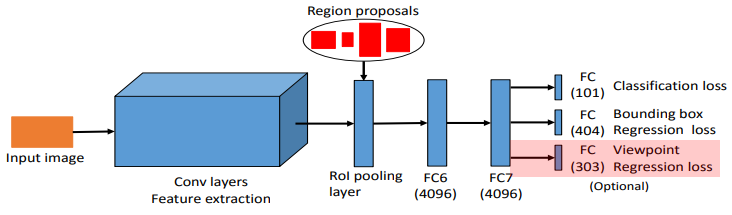
\includegraphics[width=\columnwidth]{figures/Fast-R-CNN-for-object-detection-and-pose-estimation.png}
 \caption{Fast R-CNN architecture. An image and multiple regions of interest (RoIs) are input into a convolutional
network. Each RoI is pooled into a fixed-size feature map and
then mapped to a feature vector by fully connected layers (FCs).
The network has two output vectors per RoI: softmax probabilities
and per-class bounding-box regression offsets. The architecture is
trained end-to-end with a multi-task loss, combining the losses of classification and bounding box regression.}
 \label{fig:fast-r-cnn}
\end{figure}

The 3D computer vision research community, having realised the importance of large publicly available datasets, has created a number of 3D datasets. In the lines of ImageNet, these datasets consist of images labelled, with 3D metadata such as object shape and alignment, usually by crowdsourcing or by setting HITs (Human Intelligence Tasks) in Amazon Mechanical Turk. We discuss these further in section \ref{data-and-tools}.

Large data make computer vision neural networks more robust to overfitting and better at generalising, and in line with increasing the amount of data available for training and testing to improve network performance, one common practice is data augmentation, achieved by blurring, rotating and adding noise to image subsets. Another option is to generate so called synthetic data. Generative adversarial networks (GANs) are a popular choice for creating synthetic data. In the context of 3D objects, this is also possible with open source packages such as OpenSCAD and Blender.  

The ability to generate synthetic training data, for a specific camera intrinsic matrix, with a subset of expected objects in a finite number of poses is attractive, as it constrains the computation and ultimately the size of the model, where the neural network can be designed and trained to solve a very specific problem.

We aim to replicate neural networks such as implemented by  \cite{fan2016point}. The work is seminal in bringing point clouds to the fore of 3D reconstruction, underlining the advantages of the simple and uniform structures that are easier to learn and do not have to encode multiple shape primitives or combinatorial connectivity patterns. The network outputs the point positions in a 3D frame, that is determined by the input image and the inferred viewpoint position (Figure \ref{fig:fan-et-al-vanilla}). 

\begin{figure}[ht]
 \centering 
 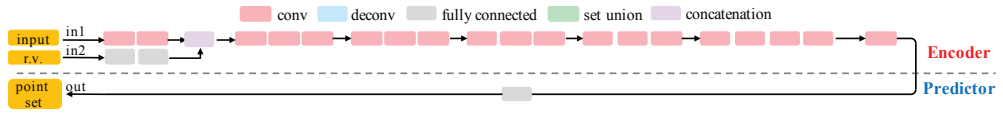
\includegraphics[width=\columnwidth]{figures/fan-et-al-vanilla.png}
 \caption{The PointOutNet \textit{vanilla} architecture}
 \label{fig:fan-et-al-vanilla}
\end{figure}

The network consists of two distinct inputs, the image input and the reference view (r.v.). The image input if followed by two convolutional layers, while the reference view if followed by two fully connected (MLP) layers. Both inputs are combined in a concatenation layer and then followed by a number of convolutional layers. This is the encoding part, where features are extracted. Finally there is a fully connected layer where a prediction (classification) is made to generate an output point set as shown in Figure \ref{fig:fan-et-al-output}. 

\begin{figure}[ht]
 \centering 
 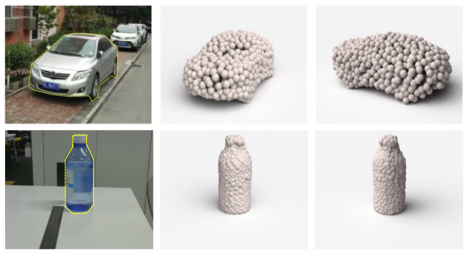
\includegraphics[width=7cm]{figures/fan-et-al-output.png}
 \caption{The PointOutNet 3D point cloud reconstruction from a single image. A segmentation mask is used to indicate the scope of the object in the input images on the left. On the right are the reconstructions viewed at 0 and 90 degrees along azimuth.  Each point is visualised as a small sphere.}
 \label{fig:fan-et-al-output}
\end{figure}

Operations performed by robots which require 3D vision, could benefit from having a compact model, optimised for the camera, generating point clouds that can be used in conjuction with LIDAR point clouds. 

We propose to develop a model prototype, that could be deployed at the embedded, desktop or cloud level. As there are many approaches but as far as we can gather, none specifically aimed at mapping image generated point clouds to be coalesced with LIDAR generated point clouds, the work involves some experimentation, replicating existing models and adapting the workflow to the specific task at hand.






%------------------
%	METHODS AND APPROACHES 
%------------------

Comprehensive description of the methods used to address the question.

\subsection{mark allocation}

iii. \textbf{Approaches -- 40\%}
\textit{show how you will undertake the work to ensure that you produce meaningful results}


\subsection{Detail Task Description} 
iii. describe the methods or approaches that you will use to answer the question effectively and robustly in some detail -- you need to show that you understand what you will do in terms of any design and build or data collection and analysis;

\subsection{Proposal Structure}

A comprehensive description of the methods used to address the question. In some cases this may involve the collection of data, consideration of its nature and details describing how it would be analysed. Note that proposals must contain descriptions of planned analysis to enable the reader (including the researcher) to determine whether any data used are suitable for the task in hand. In others it may involve a description of an appropriate software design, development and evaluation methodology. In some cases both of these will be relevant. You must also be clear about how you will ensure that you are considering relevant legal and professional issues and accounting for the emotional, physical and intellectual well-being of anyone who is effected by your study -- ethical issues must be described and discussed here with any concerns identified and addressed.

Markers will look for the extent to which approaches are: comprehensively described -- they should be documented in detail* and discussed; appropriate -- they must be aligned with the question in hand and likely to result in a successful project with robust answers; informed by existing research and practice; described in a manner that enables the reader to establish the likely quality of results; indicative of deep knowledge; specific; innovative -- where innovation in terms of approach is shown to be necessary; evaluated in terms of any limitations, assumptions or issues of scope. These criteria apply to analysis, design and research ethics.

*Students often focus on data collection rather that analysis or where 'Design \& Build' is the focus on software build and technology rather than evaluation and acquisition of knowledge in their proposals. You must demonstrate that you know how you are going to establish answers to your research question(s) through your activity including any data collection or the development of (software, hardware, prototype) artefacts. These methods should be robust in terms of process and detailed in terms of their description.

\subsection{Ethical, Legal \& Professional Issues}

Discussion of the issues that are raised and ways in which they will be addressed should be included within the main body of the proposal under 'Approaches' to demonstrate capabilities in dealing with ethical issues in the RMPI assessment. 

%------------------
%	WORK PLAN 
%------------------

\section{Work Plan}

Our work plan consists of a work breakdown structure (Figure \ref{fig:workplan}) and a Gantt chart (Figure \ref{fig:gantt-chart}).
We identified 5 principal components, each successive component has a dependency on, and cannot start before, the previous component being completed, which represents a milestone.

% Generated by https://online.visual-paradigm.com/
\begin{figure}[h]
\centering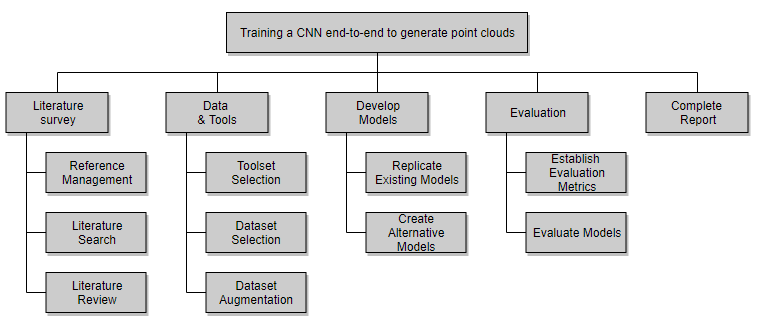
\includegraphics[width=1\linewidth]{figures/point-cloud-wbs.png}
\caption{Work breakdown structure}
\label{fig:workplan}
\end{figure}

\begin{figure}[h]
\begin{center}
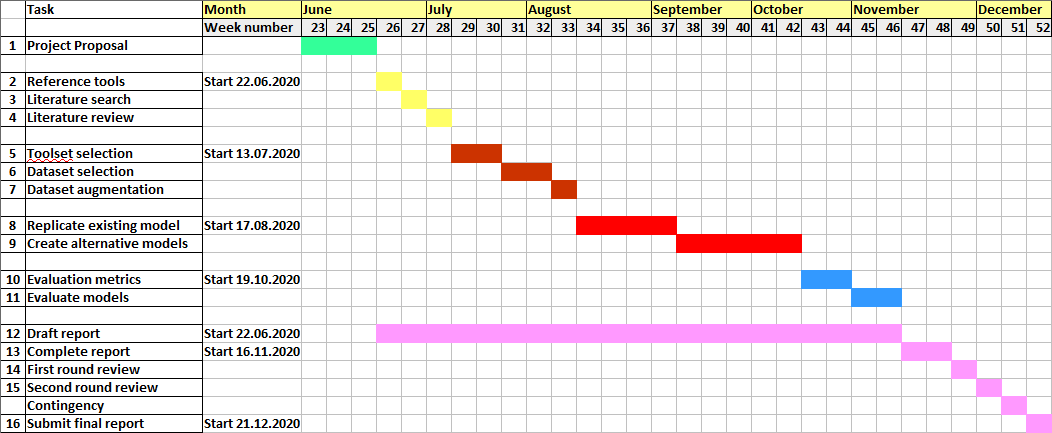
\includegraphics[scale=0.55] {figures/point-cloud-gantt-chart.png}
\caption{Gantt chart}
\label{fig:gantt-chart}
\end{center}
\end{figure}






%------------------
%	RISKS
%------------------

\section{Risks} 
\label{risks}

To generate our risk register (Table \ref{table:risk_table}), as suggested in \cite{Dawson:2009:PCI:1611433} we use: 
\begin{equation}
I = L * C
\end{equation}

where Likelihood $L$ is categorized according to three-point scale 
Low/Medium/High, Consequence $C$ according to five-point
scale Very Low/Low/Medium/High/Very High and Risk Impact $I$ is the product.
% Risk Table
% risk table cell coloring
% Manchev is the only one to apply background colouring to cells with impact above a certain score

% Colours
% red {FF0000}
% amber {FFBF00}
% green {00FF00}

% \cellcolor[HTML]{C0C0C0}
\begin{table}[h]
\begin{center}
\begin{tabular}{ |m{55mm}|m{3mm}|m{3mm}|m{5mm}|m{73mm}| } 
\hline
\textbf{Description} & \textbf{L} & \textbf{C} & \textbf{I} & \textbf{Mitigation} \\ \hline

% Insufficient knowledge
Insufficient domain knowledge
% Scores
& 2 & 4 & \cellcolor[HTML]{FFBF00} 8 &
% Mitigation
Extend scope for literature survey and toolset selection and decrease scope for alternative models \\ \hline

%% Cannot replicate all models
Cannot replicate all models in chosen environment 
& 1 & 5 & \cellcolor[HTML]{00FF00} 5 &
% Mitigation
Redefine project scope \\ \hline

% No additional networks
Unable to create synthetic data
% Scores
& 2 & 3 & \cellcolor[HTML]{FFBF00} 6 &
% Mitigation
Use existing 3D shape libraries only\\ \hline

% Sequence learning
Output point clouds too course
% Scores
& 2 & 4 & \cellcolor[HTML]{FFBF00} 8 &
% Mitigation
Use shape-to-point-cloud lookup database\\ \hline

% No additional networks
Unable to create alternative models
% Scores
& 2 & 4 & \cellcolor[HTML]{FFBF00} 8 &
% Mitigation
Use existing models only \\ \hline

% Loss of data
Accidental loss of data.
% Scores
& 2 & 5 & \cellcolor[HTML]{FF0000} 10 &
% Mitigation
Keep all source code, reporting and data online (github.com, overleaf.com, aws.amazon.com, camber.city.ac.uk and devcloud.intel.com) \\ \hline
%Keep source code repository on github.com, project report on overleaf.com 
%and data on aws.amazon.com

%% COVID
% Description
Continued COVID-19 lockdown disruption
& 2 & 3 & \cellcolor[HTML]{FFBF00} 6 &
% Mitigation
Scale down project \\ \hline

% Report writing overruns
Final report delay 
% Scores
& 2 & 5 & \cellcolor[HTML]{FF0000} 10 & 
% Mitigation
One additional week has been added for contingency \\ \hline
\end{tabular}
\end{center}
\caption{Risk register}
\label{table:risk_table}
\end{table}

%\lipsum[1]
%\lipsum[2]

%------------------
%	RESEARCH ETHICS & PROFESSIONAL ISSUES
%------------------

\section{Ethical, Legal and Professional Issues}
Having completed \textit{Part A: Ethics Checklist} of the Research Ethics Review Form, as determined by the Computer Science Research Ethics Committee (\cite{CSREC:2020}), we find this work complies with research ethics guidelines and does not require ethical approval.





%------------------
%	REFERENCES
%------------------

% References in separate page
%% we use \clearpage to achieve the effect of \pagebreak
%% https://tex.stackexchange.com/questions/234057/pagebreak-newpage-vspace-all-not-working-after-a-table
\clearpage
\printbibliography


%------------------
%	RESEARCH ETHICS REVIEW FORM
%------------------

% Better results obtained using https://pdfjoiner.com/
% join completed-ethics-form.pdf
% \GitHub\msc-data-science\INM363-IndividualProjects\coursework

% 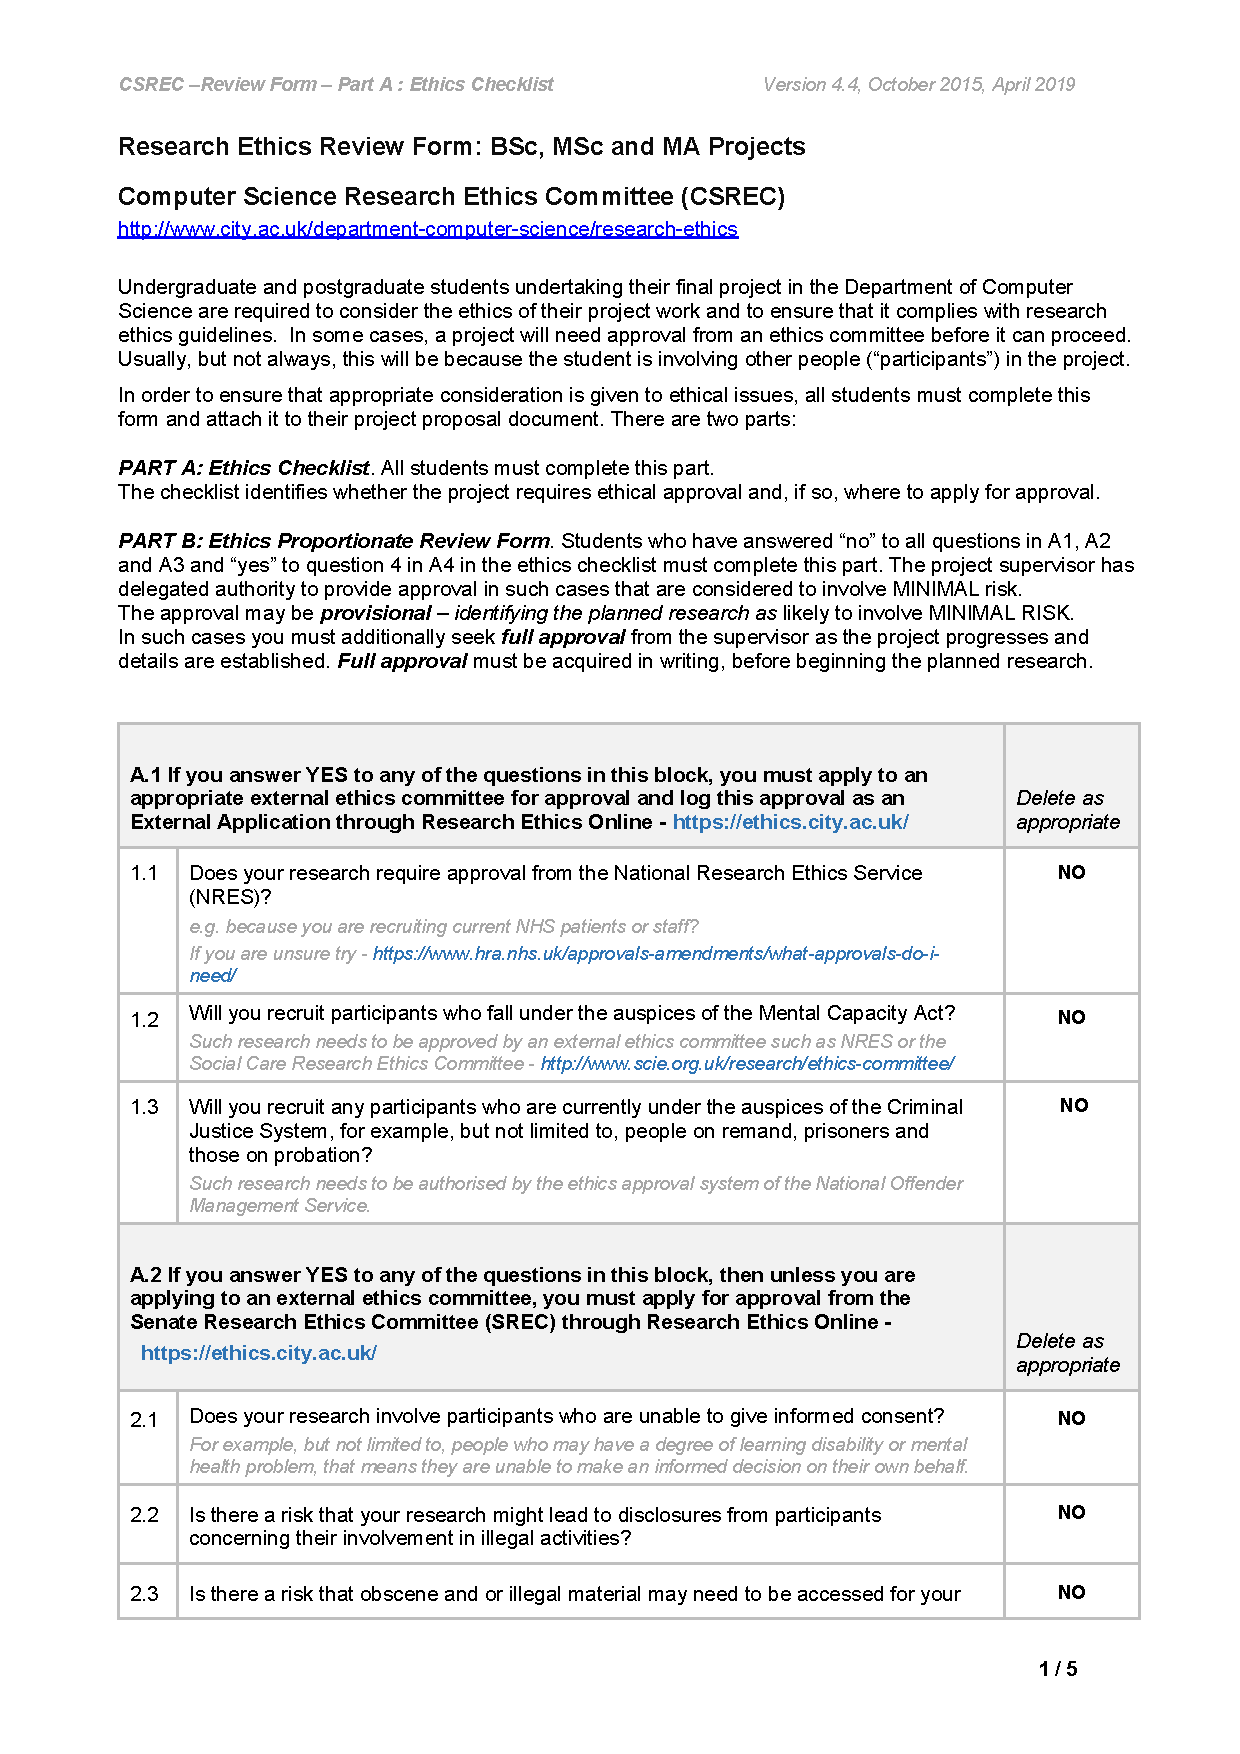
\includepdf[pages=-,pagecommand={},width=\linewidth]{ethics-form.pdf}

\end{document}